\documentclass[conference,11pt]{IEEEtran}

\usepackage[T1]{fontenc}
\usepackage[utf8]{inputenc}
\usepackage[french]{babel}
\usepackage{graphicx}
\usepackage{booktabs}
\usepackage{array}
\usepackage{url}
\usepackage{microtype}

\graphicspath{{figures/}}

\title{Étude comparative des performances d'une application web de gestion de bibliothèque développée en PHP, Node.js, Python et Java}

\author{
\IEEEauthorblockN{Kintaudi Ndinda Benjamine}
\IEEEauthorblockA{FASI, UPC\\
\texttt{benjaminendinda@gmail.com}}
\and
\IEEEauthorblockN{Lisongo Ekonzo Catherine}
\IEEEauthorblockA{FASI, UPC\\
\texttt{lisongocathy8@gmail.com}}
\and
\IEEEauthorblockN{Inaka La Joie La Joie}
\IEEEauthorblockA{FASI, UPC\\
\texttt{Inakalajoie@gmail.com}}
\and
\IEEEauthorblockN{Mona Elameji Pauline}
\IEEEauthorblockA{FASI, UPC\\
\texttt{Paulelameji@gmail.com}}
\and
\IEEEauthorblockN{Lomami Ekanga Nana}
\IEEEauthorblockA{FASI, UPC\\
\texttt{djulianalomami3@gmail.com}}
}

\begin{document}

\maketitle

\begin{abstract}
Ce travail compare quatre applications indépendantes d'une même
mini-bibliothèque, réalisées avec PHP, Node.js, Python et Java. Nous mesurons
le temps de réponse HTTP de leur page d'accueil pour quatre niveaux de
concurrence : 1, 5, 10 et 20. Après cinq requêtes de préchauffage, trente
requêtes sont mesurées pour chaque couple technologie--concurrence.
À concurrence 20, les médianes sont de 82,836~ms pour PHP, 55,290~ms pour
Node.js, 135,790~ms pour Python et 35,395~ms pour Java. Ces valeurs décrivent
une expérience de bout en bout : elles ne permettent donc pas d'attribuer
isolément les écarts au langage utilisé.
\end{abstract}

\begin{IEEEkeywords}
benchmark HTTP, concurrence, temps de réponse, PHP, Node.js, Flask, Spring Boot
\end{IEEEkeywords}

\section{Introduction}

La performance observable d'une application web compte pour les utilisateurs
qui attendent une réponse rapide, notamment lorsque plusieurs requêtes
arrivent simultanément. Les effets des requêtes lentes peuvent être amplifiés
à l'échelle d'un service distribué, ce qui justifie de distinguer la médiane
des mesures de queue de distribution \cite{tail}. Les comparaisons entre langages et frameworks sont
cependant difficiles : le résultat dépend aussi du serveur HTTP, du code
applicatif, des accès aux données, de la machine et de la charge.

Ce travail étudie une question précise : comment le temps de réponse médian de
la page d'accueil évolue-t-il lorsque la concurrence passe de 1 à 20 requêtes
pour quatre implémentations d'une mini-bibliothèque ? L'hypothèse explorée
est que la concurrence augmente le temps de réponse, mais que l'ampleur de
cette augmentation dépend de chaque pile technique.

La contribution est un protocole HTTP reproductible, ses mesures synthétisées
et une discussion prudente des écarts. La section II décrit la méthodologie,
la section III le développement et l'équivalence des versions, la section IV
les résultats, puis la section V conclut l'étude.

\section{Méthodologie}

\subsection{Application de référence}

BiblioQuad regroupe quatre applications indépendantes de mini-bibliothèque.
Le cahier des charges fonctionnel porte sur la gestion de livres,
d'emprunteurs et d'emprunts. Le schéma décrit dans le projet contient
\texttt{livres(id, titre, auteur, categorie, quantite)},
\texttt{emprunteurs} et \texttt{emprunts}. Les quatre applications exposent
une page d'accueil accessible par HTTP. Le test étudié ici n'exécute que
\texttt{GET /} et ne modifie ni application ni base de données.

\subsection{Technologies comparées}

Les versions observées dans l'environnement de travail et les contraintes
déclarées par le projet sont reportées séparément dans le
tableau~\ref{tab:technologies}. Cette distinction évite de transformer une
plage de dépendance en version effectivement installée.

\begin{table}[!t]
\centering
\caption{Technologies comparées}
\label{tab:technologies}
\footnotesize
\begin{tabular}{p{0.20\columnwidth}p{0.27\columnwidth}p{0.36\columnwidth}}
\toprule
Technologie & Version observée & Projet / dépendance déclarée \\
\midrule
PHP & PHP 8.5.3 & non indiquée \\
Node.js & Node.js 26.13.1; Express 4.22.3 & \texttt{\string^4.21.2} \\
Python & Python 3.12.10; Flask 3.1.3 & Flask $\geq$ 3.0, $<4$ \\
Java & Java 25.0.5 LTS & Java 21 déclaré; Spring Boot 3.4.1 \\
\bottomrule
\end{tabular}
\end{table}

Les versions observées ci-dessus ont été relevées dans l'environnement de
travail lors de la finalisation de l'article. Le fichier de synthèse ne
contient pas d'empreinte de versions permettant de prouver qu'elles sont
identiques à celles de la campagne HTTP ; cette limite est conservée dans
l'interprétation.

\subsection{Métriques}

La durée est le temps écoulé entre le début d'une requête et la lecture
complète de sa réponse, exprimé en millisecondes. Elle est mesurée avec
\texttt{time.perf\_counter\_ns()}, une horloge monotone documentée par Python
\cite{python-time}. Pour chaque
configuration, le fichier de synthèse contient la moyenne, la médiane, le
95\textsuperscript{e} percentile, le taux d'erreur et le débit en requêtes par seconde.
La médiane résume la position centrale des trente durées et limite
l'influence des valeurs extrêmes ; le 95\textsuperscript{e} percentile décrit la durée
atteinte par la grande majorité des requêtes. Le temps moyen complète cette
lecture robuste, tandis que le débit résume la quantité de requêtes achevées
pendant la phase de mesure. La nécessité d'un protocole statistiquement
rigoureux pour comparer des exécutions est également soulignée dans
\cite{georges}.

Le taux d'erreur compte les exceptions réseau, les dépassements de délai et
les codes HTTP finaux hors de l'intervalle 200--399. Le débit est calculé sur
la durée murale de la phase mesurée. Dans les résultats étudiés, le taux
d'erreur est nul pour toutes les configurations.

\subsection{Outils et environnement de test}

Le lanceur \texttt{benchmark\_http.py} utilise Python et \texttt{aiohttp},
une bibliothèque cliente et serveur HTTP asynchrone pour \texttt{asyncio}
\cite{aiohttp}.
Les pages d'accueil ont été adressées aux URL locales suivantes : PHP sur
le port 8000, Node.js sur 3000, Python sur 5000 et Java sur 8080. Le délai
d'expiration total du client est de 10 secondes. Les résultats utilisés dans
cet article proviennent de
\texttt{resultats\_http\_synthese.csv}; les graphiques sont ceux
générés à partir de ce fichier.

\subsection{Déroulement des tests}

Les applications sont testées successivement afin de limiter les
interférences. Pour chaque technologie et chaque niveau de concurrence
(1, 5, 10 et 20), cinq requêtes d'échauffement sont d'abord envoyées et
exclues des statistiques. Trente requêtes sont ensuite mesurées. Chaque
tentative est enregistrée avec sa technologie, sa concurrence, son numéro,
sa durée, son code HTTP et son éventuelle erreur. Cette organisation permet
à un autre groupe de reproduire le même protocole sans envoyer de requête
d'écriture.
Les requêtes d'une même phase sont regroupées par lots limités par le niveau
de concurrence demandé. Ainsi, le niveau 1 produit une exécution séquentielle
et les niveaux supérieurs permettent plusieurs requêtes simultanées, sans
dépasser la valeur configurée. Les réponses sont lues jusqu'à leur fin avant
d'arrêter chaque chronomètre : le benchmark mesure la réponse HTTP complète
et non le seul moment où les en-têtes sont reçus.

\section{Développement}

\subsection{Réalisation des versions}

La version PHP est une application MVC native, dans l'écosystème documenté
par le manuel officiel PHP \cite{php-manual}. La version Node.js repose sur
Express et le moteur de vues EJS ; l'API HTTP de Node.js fournit notamment
les interfaces serveur et client bas niveau \cite{node-http}. La version
Python utilise Flask, framework WSGI léger décrit dans sa documentation
officielle \cite{flask}. La version Java est une application Spring Boot avec
Thymeleaf et JDBC ; Spring Boot documente la création d'applications Java
autonomes et orientées production \cite{spring-boot}. Les quatre
applications utilisent MySQL dans leur architecture, mais leurs pilotes,
serveurs d'application et chemins de rendu restent propres à chaque
implémentation.

\subsection{Équivalence fonctionnelle}

L'équivalence visée concerne le domaine fonctionnel et la requête HTTP
comparée : chaque application est sollicitée par un \texttt{GET /} sur sa
propre URL locale. Le benchmark ne modifie pas les données et ne compare pas
des requêtes SQL internes. Les pages d'accueil n'étant pas garanties
identiques instruction par instruction, l'équivalence est comportementale
pour le scénario retenu et non une isolation parfaite du langage.

\subsection{Difficultés rencontrées}

Les difficultés techniques vérifiables ont d'abord été l'harmonisation de
quatre applications qui n'utilisent ni le même serveur ni le même framework :
les pages d'accueil sont exposées sur quatre ports et les connexions MySQL
sont configurées séparément. Le client de mesure a donc dû limiter son
scénario à \texttt{GET /}, conserver une session HTTP par application et
exécuter les applications successivement.

Une seconde difficulté vient de la gestion des versions : le dépôt déclare
des plages pour certaines dépendances, tandis que l'environnement possède des
versions installées précises ; le projet Java déclare Java 21 alors que le
runtime observé est Java 25.0.5. Cette différence est signalée dans le
tableau au lieu d'être masquée. Enfin, la page d'accueil n'a pas un traitement
interne garanti identique dans les quatre applications. Le protocole rend
comparables la requête, la concurrence et la mesure, mais ne supprime pas les
différences de rendu, de cache, de connexion à MySQL ou d'ordonnancement du
système.

\section{Résultats et discussion}

\subsection{Données recueillies}

Le tableau~\ref{tab:mesures} reprend les valeurs du CSV à concurrence 20.
Les temps sont en millisecondes, le taux d'erreur est une proportion et le
débit est exprimé en requêtes par seconde.

\begin{table}[!t]
\centering
\caption{Synthèse des mesures à concurrence 20}
\label{tab:mesures}
\scriptsize
\begin{tabular}{lrrrrr}
\toprule
Technologie & Moy. & Méd. & P95 & Erreur & Débit \\
 & ms & ms & ms & & req/s \\
\midrule
PHP & 76,235 & 82,836 & 101,622 & 0 & 180,320 \\
Node.js & 48,990 & 55,290 & 70,894 & 0 & 316,633 \\
Python & 133,547 & 135,790 & 181,838 & 0 & 116,468 \\
Java & 51,091 & 35,395 & 91,131 & 0 & 299,340 \\
\bottomrule
\end{tabular}
\end{table}

Les médianes complètes sont les suivantes : à concurrence 1, PHP obtient
5,256~ms, Node.js 6,982~ms, Python 10,986~ms et Java 10,454~ms ; à
concurrence 5, elles valent respectivement 23,403, 15,411, 39,868 et
13,464~ms ; à concurrence 10, 48,307, 46,855, 82,426 et 25,324~ms ; enfin,
à concurrence 20, 82,836, 55,290, 135,790 et 35,395~ms.

\begin{table}[!t]
\centering
\caption{Médianes selon les quatre niveaux de concurrence}
\label{tab:medians}
\footnotesize
\begin{tabular}{lrrrr}
\toprule
Technologie & 1 & 5 & 10 & 20 \\
\midrule
PHP & 5,256 & 23,403 & 48,307 & 82,836 \\
Node.js & 6,982 & 15,411 & 46,855 & 55,290 \\
Python & 10,986 & 39,868 & 82,426 & 135,790 \\
Java & 10,454 & 13,464 & 25,324 & 35,395 \\
\bottomrule
\end{tabular}
\end{table}

Le tableau~\ref{tab:medians} permet de comparer les quatre technologies
sur toute la campagne plutôt qu'à la seule charge maximale. Il met aussi en
évidence que la valeur à concurrence 20 ne suffit pas à décrire la réponse
à faible charge : à concurrence 1, PHP est la technologie dont la médiane
est la plus faible dans les données fournies, alors qu'à concurrence 20 la
plus faible médiane est celle de Java.

\subsection{Analyse}

La figure~\ref{fig:barres} montre qu'à concurrence 20 la médiane Java est la
plus faible des quatre, tandis que Python est la plus élevée. Node.js et PHP
occupent des positions intermédiaires. Le classement porte uniquement sur
la page et l'environnement de l'expérience.

\begin{figure}[!t]
\centering
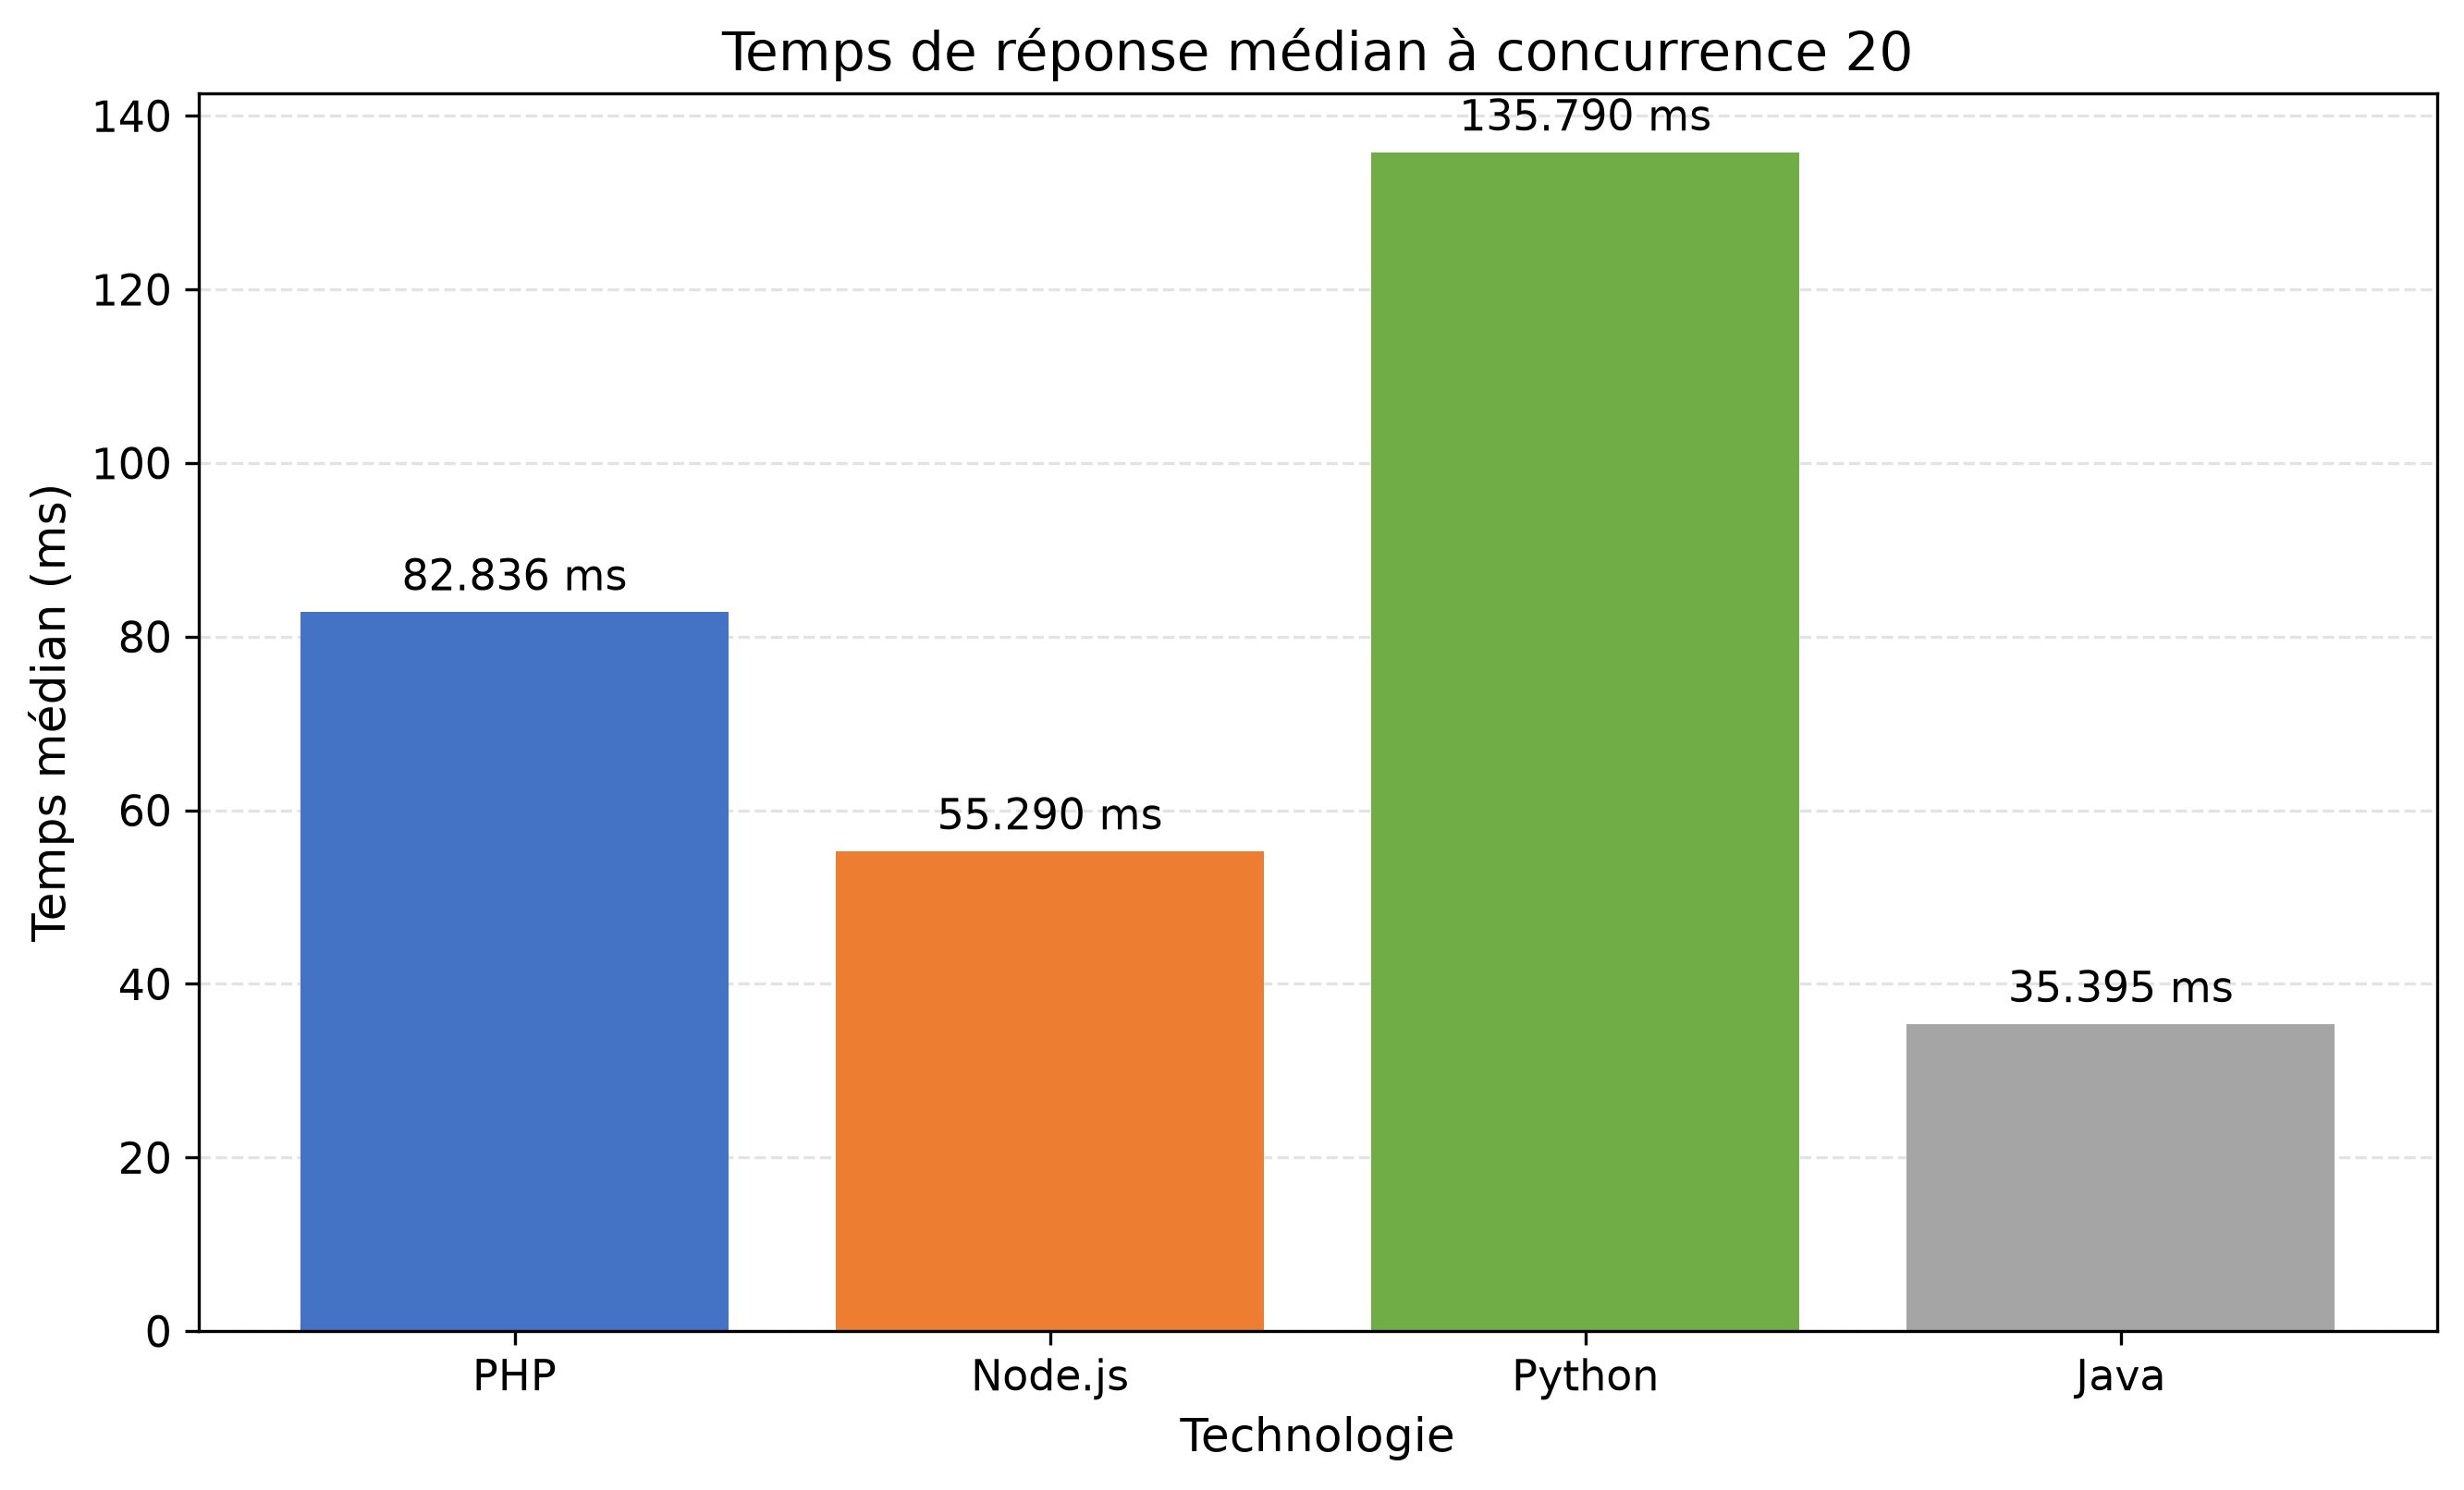
\includegraphics[width=\columnwidth]{temps_medians_concurrence_20.png}
\caption{Temps de réponse médian à concurrence 20.}
\label{fig:barres}
\end{figure}

La figure~\ref{fig:lignes} montre une hausse globale des médianes avec la
concurrence, mais avec des pentes différentes. La médiane Node.js passe de
6,982~ms à concurrence 1 à 15,411~ms à concurrence 5 ; cette variation
reste compatible avec une hausse non linéaire et rappelle que les mesures
réelles fluctuent.

\begin{figure}[!t]
\centering
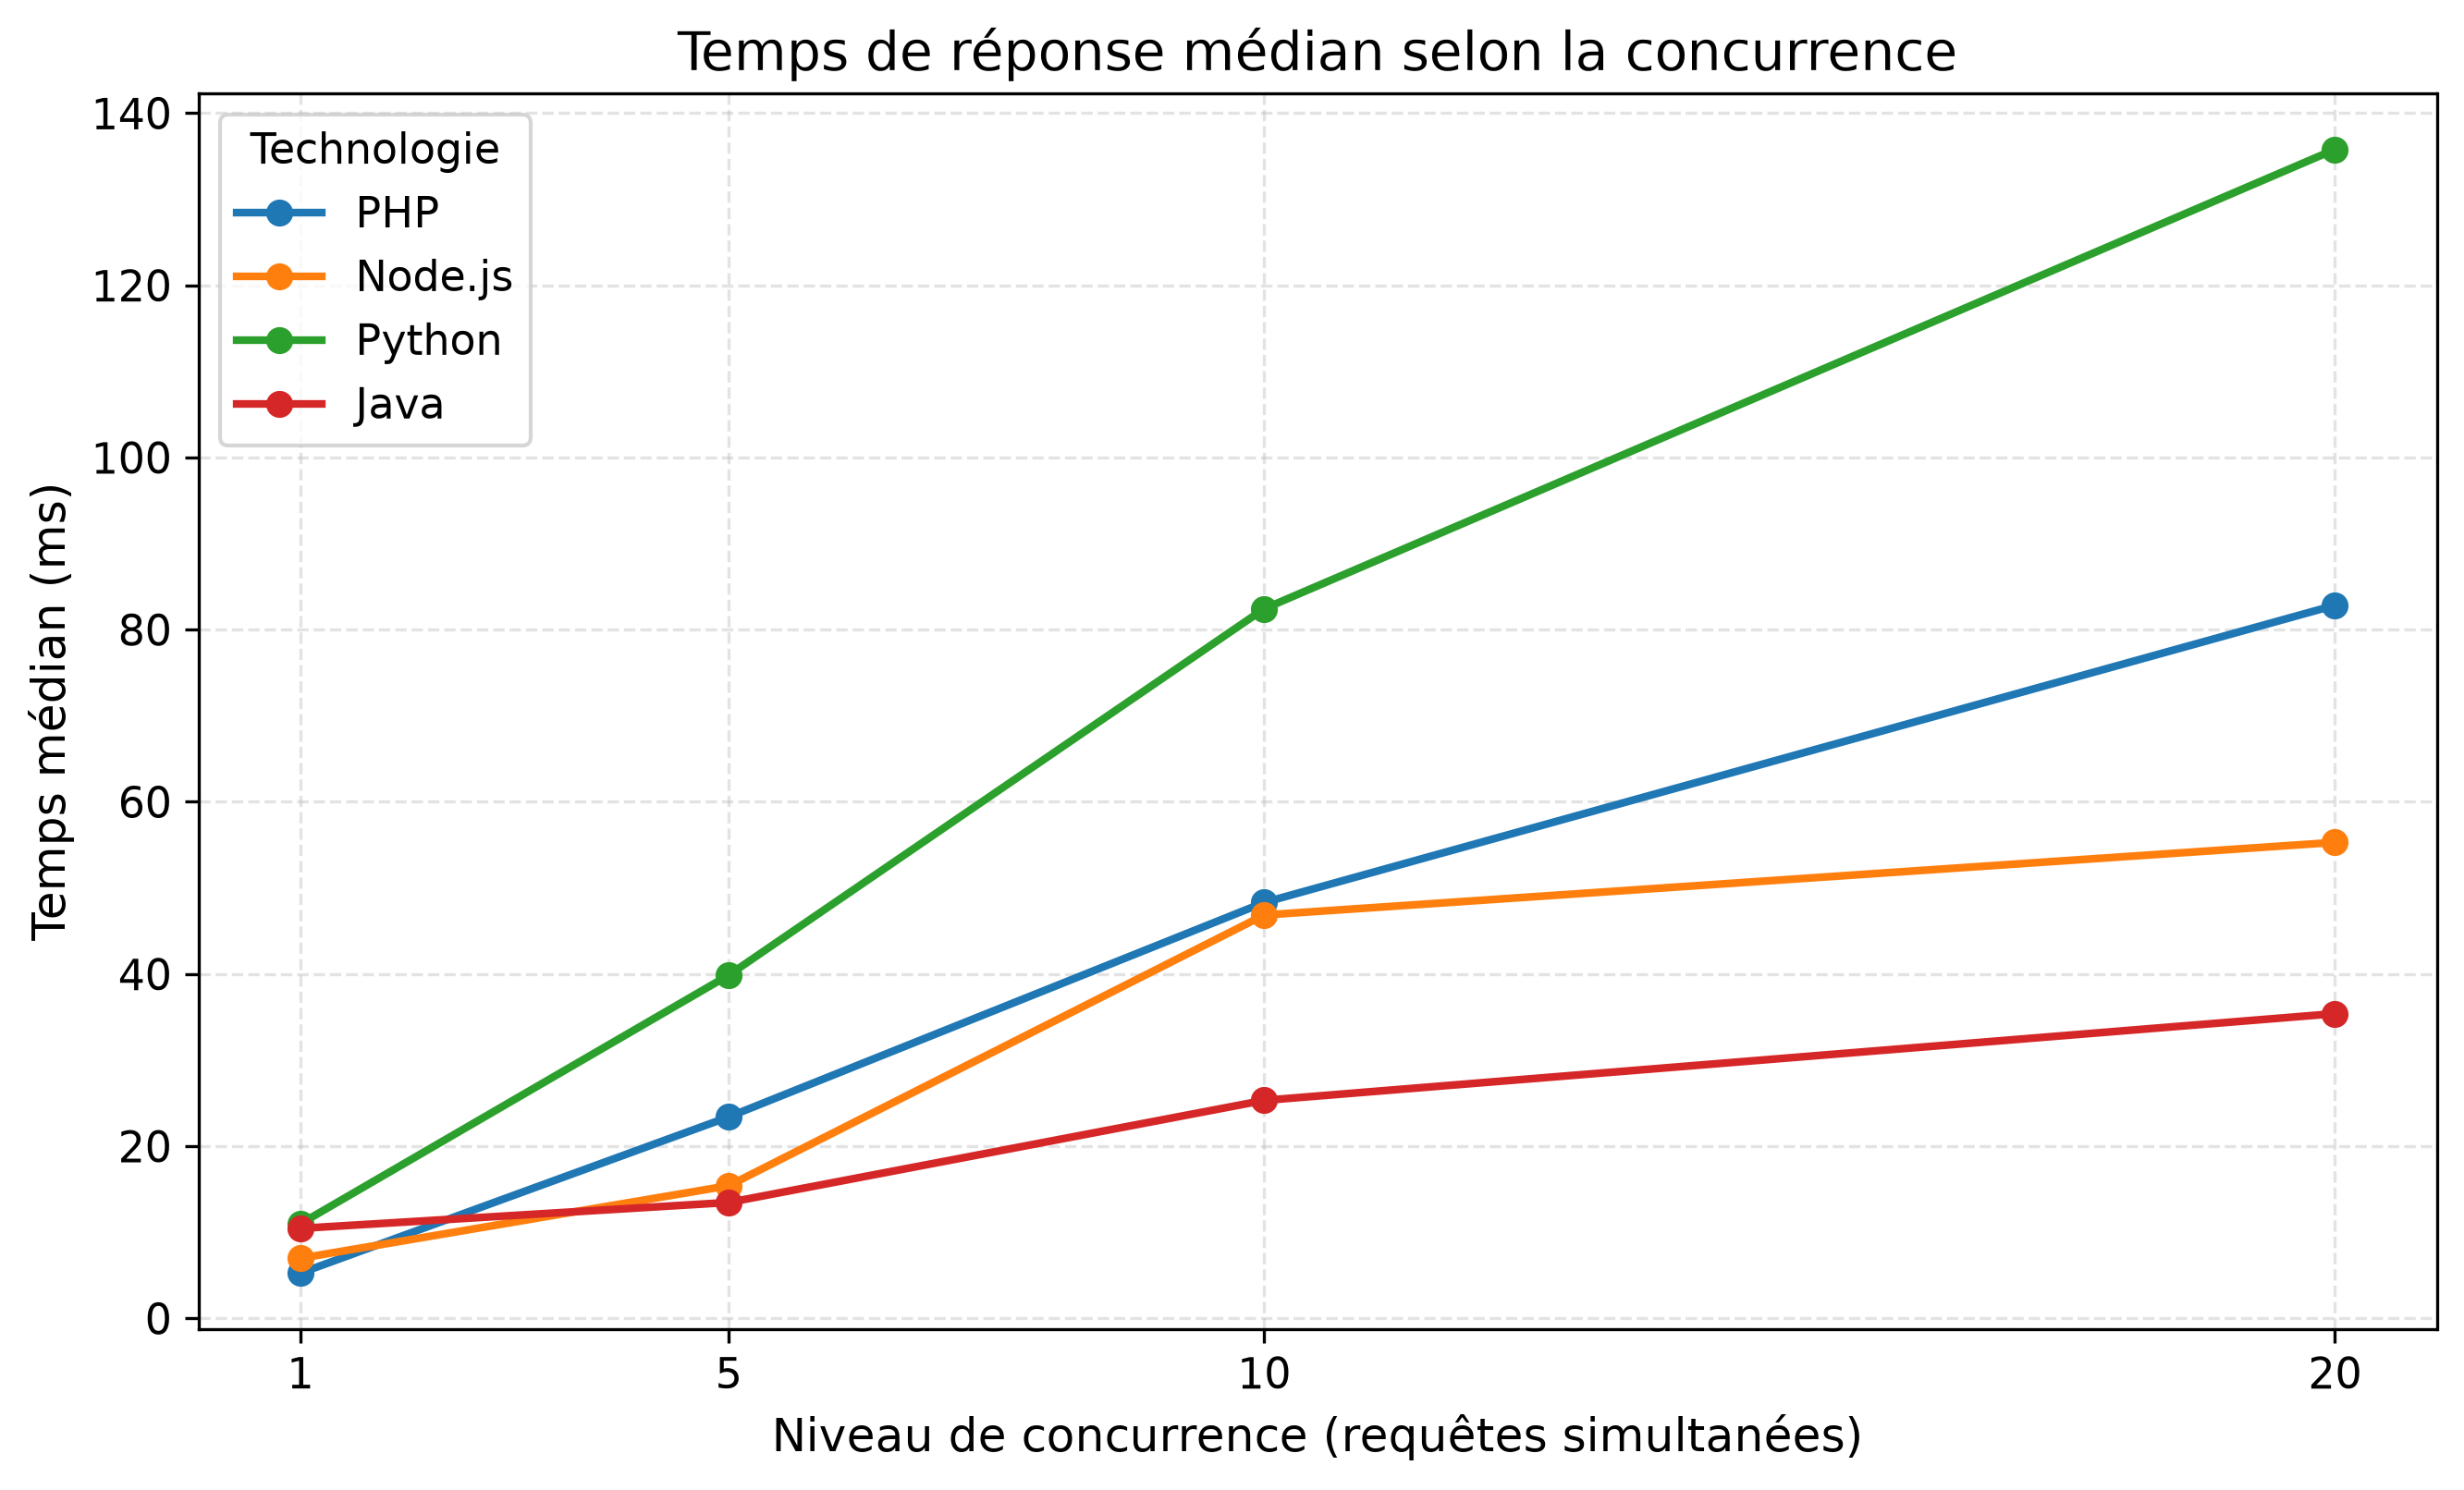
\includegraphics[width=\columnwidth]{temps_medians_par_concurrence.png}
\caption{Temps de réponse médian selon la concurrence.}
\label{fig:lignes}
\end{figure}

\subsection{Interprétation et discussion}

Les données sont compatibles avec l'hypothèse d'une dégradation lorsque la
concurrence augmente, surtout pour Python dans cette campagne. Elles ne
permettent pas de conclure qu'un langage est intrinsèquement plus rapide.
Le temps HTTP inclut le client, le serveur, le routage, le rendu, les accès
éventuels à MySQL, le réseau local et la lecture de la réponse. Les pages
d'accueil peuvent effectuer des traitements internes différents ; le test
n'est donc pas une comparaison parfaitement isolée des langages.

La durée médiane et le débit ne doivent pas être confondus : à concurrence
20, Node.js présente un débit de 316,633~requêtes/s dans le CSV, alors que
sa médiane est de 55,290~ms. Ces indicateurs répondent à des questions
différentes et doivent être interprétés ensemble. Cette lecture des valeurs
de queue est cohérente avec l'importance de la variabilité de latence
décrite par Dean et Barroso \cite{tail}.

Le 95\textsuperscript{e} percentile suit également cette distinction. À concurrence 20,
les valeurs indiquées dans le CSV sont 101,622~ms pour PHP, 70,894~ms pour
Node.js, 181,838~ms pour Python et 91,131~ms pour Java. La médiane décrit
le centre de la distribution, tandis que le percentile rend visibles les
requêtes plus lentes. Dans cette campagne, aucune erreur HTTP ou réseau n'a
été comptabilisée pour modifier ces indicateurs.

Il faut également distinguer l'équité du protocole et l'identité de
l'implémentation. L'équité vient des mêmes nombres de requêtes, de la même
horloge, des mêmes niveaux de concurrence et du même traitement des erreurs.
L'identité ne peut pas être affirmée, car chaque application utilise son
propre serveur, son propre framework et potentiellement son propre chemin
d'accès aux données. Le protocole rend cette différence explicite au lieu de
la masquer derrière un classement unique.

\section{Conclusion}

L'étude répond à la question posée en observant l'évolution des temps
médians HTTP pour quatre applications et quatre niveaux de concurrence. Dans
le jeu de données fourni, Java a la médiane la plus faible à concurrence 20
(35,395~ms) et Python la plus élevée (135,790~ms). La réponse doit rester
limitée à cette page d'accueil, cette machine, cette configuration et cette
campagne de trente mesures.

Une suite utile serait de répéter plusieurs campagnes, de contrôler
explicitement les versions d'exécution, puis de mesurer séparément le temps
du serveur HTTP, du code applicatif et de la base de données. Cette
décomposition permettrait de mieux expliquer les écarts sans les attribuer
directement aux seuls langages.

Une autre extension consisterait à conserver, pour chaque campagne, les
mesures brutes et les informations de contexte : état de la machine, charge
des services, versions exactes des interpréteurs et taille des réponses.
Ces informations permettraient de vérifier la stabilité des médianes et
d'identifier les valeurs aberrantes avant toute comparaison entre campagnes.

\section*{Utilisation de l'intelligence artificielle}

L'intelligence artificielle a aidé à inspecter le projet, à formaliser le
protocole HTTP, à produire le lanceur et les graphiques, puis à restructurer
cet article selon le modèle fourni. Les mesures et toutes les valeurs
rapportées proviennent du fichier
\texttt{resultats\_http\_synthese.csv}; aucune mesure n'a été inventée.
La vérification du contenu, l'interprétation scientifique et la
responsabilité du document final restent celles de l'équipe.

\begin{thebibliography}{00}

\bibitem{php-manual}
The PHP Documentation Group, ``PHP Manual.'' [En ligne]. Disponible :
\url{https://www.php.net/manual/en/}. [Consulté le 16 novembre 2026].

\bibitem{node-http}
Node.js contributors, ``HTTP | Node.js Documentation.'' [En ligne].
Disponible : \url{https://nodejs.org/api/http.html}.
[Consulté le 16 novembre 2026].

\bibitem{flask}
Pallets Projects, ``Welcome to Flask --- Flask Documentation (3.1.x).''
[En ligne]. Disponible : \url{https://flask.palletsprojects.com/en/stable/}.
[Consulté le 16 novembre 2026].

\bibitem{spring-boot}
The Spring team, ``Spring Boot Reference Documentation.'' [En ligne].
Disponible :
\url{https://docs.spring.io/spring-boot/}.
[Consulté le 16 novembre 2026].

\bibitem{python-time}
Python Software Foundation, ``time --- Time access and conversions.''
[En ligne]. Disponible :
\url{https://docs.python.org/3/library/time.html#time.perf_counter_ns}.
[Consulté le 16 novembre 2026].

\bibitem{aiohttp}
aiohttp contributors, ``Welcome to AIOHTTP.'' [En ligne]. Disponible :
\url{https://docs.aiohttp.org/en/stable/}.
[Consulté le 16 novembre 2026].

\bibitem{georges}
A. Georges, D. Buytaert, and L. Eeckhout, ``Statistically rigorous Java
performance evaluation,'' in \emph{Proceedings of the 22nd annual ACM
SIGPLAN conference on Object-oriented programming systems, languages, and
applications}, 2007, pp. 57--76, doi:
\url{https://doi.org/10.1145/1297027.1297033}.

\bibitem{tail}
J. Dean and L. A. Barroso, ``The tail at scale,'' \emph{Communications of
the ACM}, vol. 56, no. 2, pp. 74--80, 2013, doi:
\url{https://doi.org/10.1145/2408776.2408794}.

\end{thebibliography}

\end{document}
